\chapter{istar: Software as a Service}

Having released and advertised idock, we kept receiving constant docking requirements from our colleges and collaborators. They are mostly biochemists and pharmacists, outsourcing the docking research to us after discovering potential biological targets for certain diseases of therapeutic interest. All of a sudden, we had to grab the protein structure, do format conversion, define search space, set up docking parameters, and keep running idock for months. Occasionally we also had to restart virtual screening in case the idock process got killed by others or by exceptions. Tedious enough, all the above work was done manually, resulting in very low research productivity.

We propose istar, a SaaS (Software as a Service) platform. The original goal of istar was to automate the virtual screening process. Now we are constructing istar as a general SaaS platform for any programs including idock \citep{1153} and igrep \citep{1138}. Without tedious software installation, users, especially computational chemists, can submit jobs on the fly either by browsing our web site (Figures \ref{istar:istar}, \ref{istar:idock} and \ref{istar:igrep}) or by programming against our RESTful API (Figure \ref{istar:RESTfulAPI}).

\begin{figure}
\centering
\includegraphics[width=\linewidth]{istar/istar.png}
\caption{http://istar.cse.cuhk.edu.hk}
\label{istar:istar}
\end{figure}

\begin{figure}
\centering
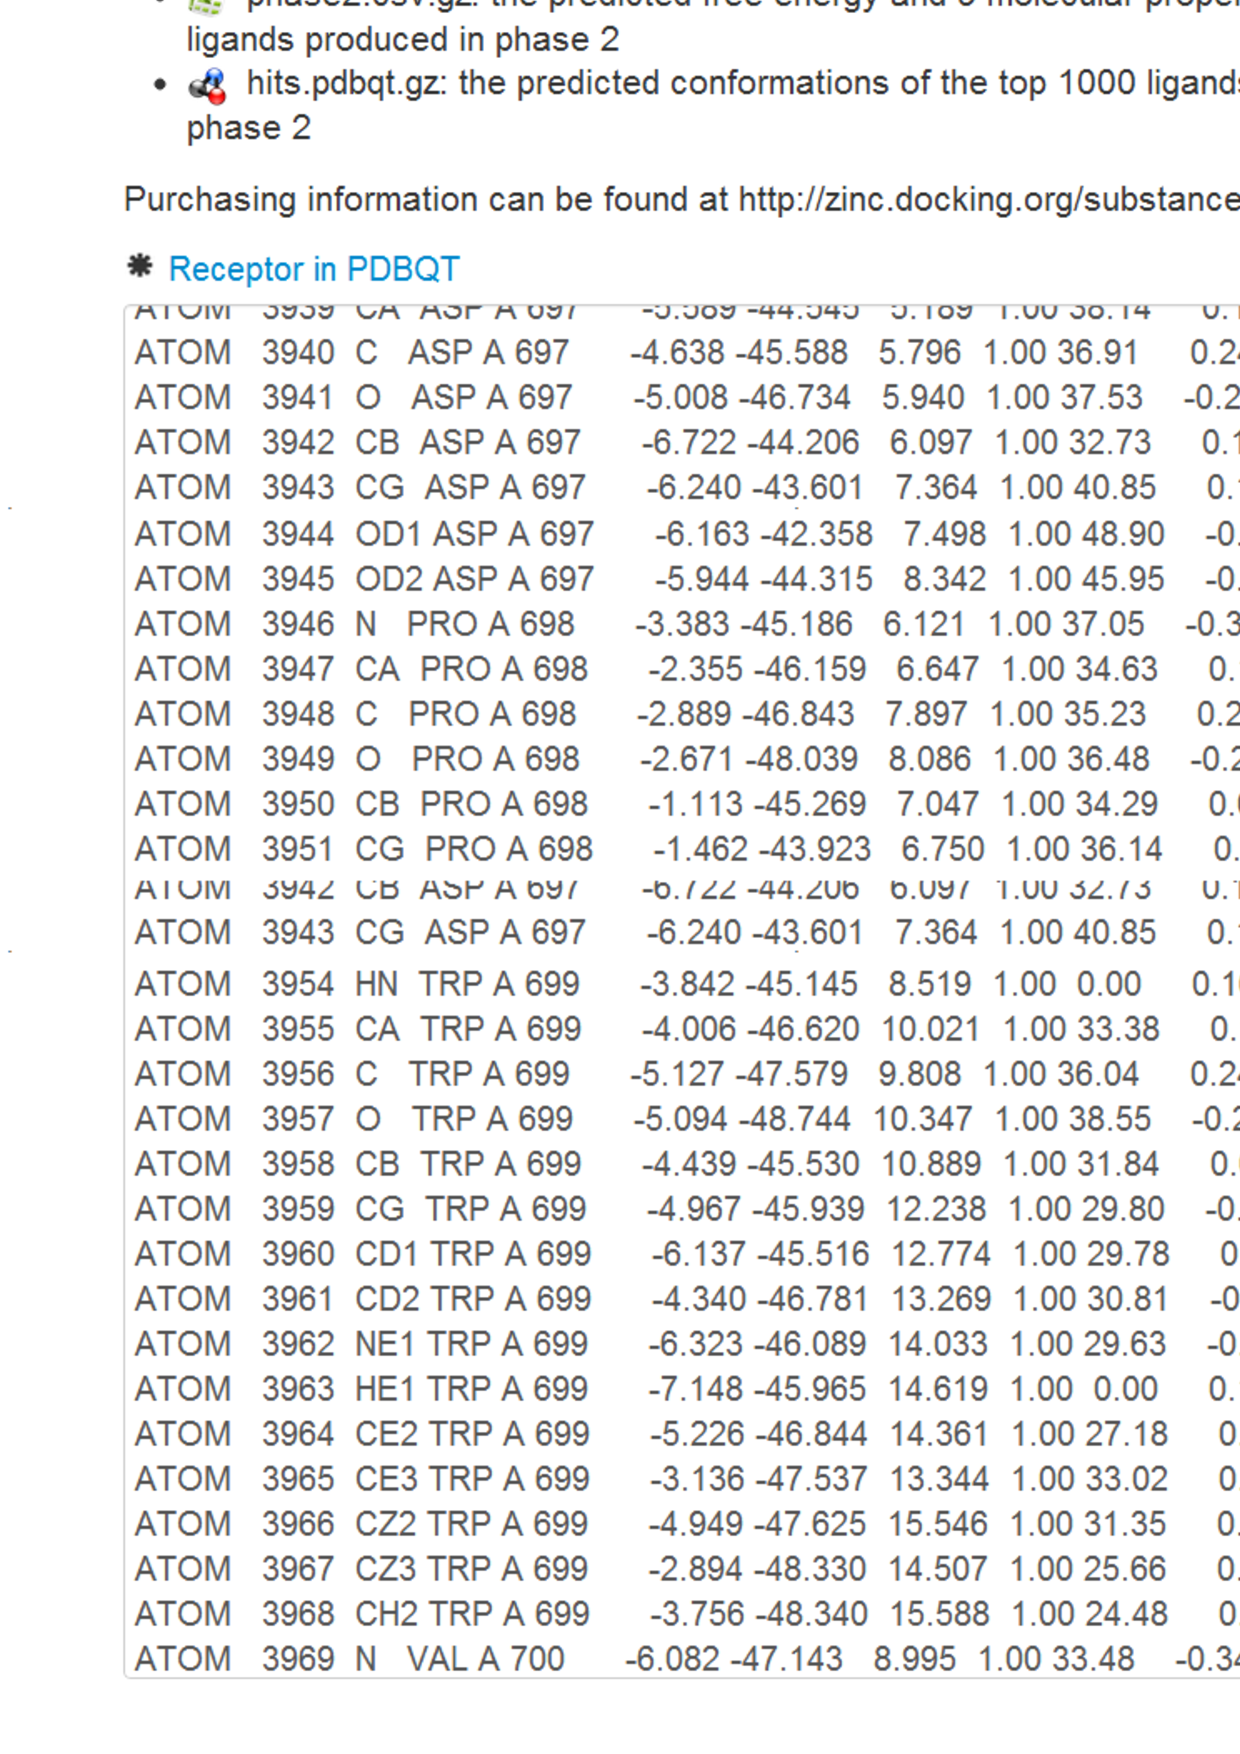
\includegraphics[width=\linewidth]{istar/idock.png}
\caption{http://idock.cse.cuhk.edu.hk}
\label{istar:idock}
\end{figure}

\begin{figure}
\centering
\includegraphics[width=\linewidth]{istar/igrep.png}
\caption{http://igrep.cse.cuhk.edu.hk}
\label{istar:igrep}
\end{figure}

\begin{figure}
\centering
\includegraphics[width=\linewidth]{istar/RESTfulAPI.png}
\caption{RESTful API for idock and igrep.}
\label{istar:RESTfulAPI}
\end{figure}

Figure \ref{istar:istar} shows the architecture of istar. On the client side, we seamlessly combine both the Twitter Bootstrap and the HTML5 Boilerplate into a HTML5- and CSS3-powered web site. We use the Modernizr JavaScript library to detect HTML5 and CSS3 features in order to maintain backward compatibility in older browsers. We adopt the \textit{de facto} jQuery JavaScript library to simplify HTML document traversing, event handling, animating, and Ajax interactions. We test the user interface on Google Chrome 19+, Mozilla Firefox 12+, Microsoft Internet Explorer 9+ and Apple Safari 5+.

On the server side, we build the web server in the same JavaScript language using the well-known asynchronous event-driven node.js on top of the express server, forking multiple worker processes to accept simultaneous HTTP connections. During startup, the master process loads and parses 9 molecular properties of 12 million ligands (Figure \ref{istar:LigandProperties}), and awaits queries from worker processes through inter-process message passing. Upon receival of a query from a worker process, the master process performs an in-memory table scan and calculates the number of ligands satisfying a given combination of filtering conditions on those 9 molecular properties. The ligand count was signaled to the query-invoking worker process and then forwarded to the client side. The entire round trip costs approximately one second, rendering the feasibility of real-time ligand counting queries for users to estimate in advance how many ligands will be docked. We expose the functionalities of job submission, job query, and ligand counting as RESTful API for others to program against. We employ the forever utility for the web server to automatically restart processes in case of unhandled exceptions, ensuring failover and high availability. We are meanwhile considering prepending the scalable asynchronous event-driven nginx as a front-end HTTP server for a rich set of features, like bandwidth throttling, static file serving, reverse proxy for caching, load balancing, URL rewriting, gzip compression, TLS/SSL support, IP-based geolocation, etc.

\begin{figure}
\centering
\subfloat
{
  \includegraphics[width=0.315\linewidth]{istar/MWT.pdf}
}
\subfloat
{
  \includegraphics[width=0.315\linewidth]{istar/LogP.pdf}
}
\subfloat
{
  \includegraphics[width=0.315\linewidth]{istar/Desolv_apolar.pdf}
}
\\
\subfloat
{
  \includegraphics[width=0.315\linewidth]{istar/Desolv_polar.pdf}
}
\subfloat
{
  \includegraphics[width=0.315\linewidth]{istar/HBD.pdf}
}
\subfloat
{
  \includegraphics[width=0.315\linewidth]{istar/HBA.pdf}
}
\\
\subfloat
{
  \includegraphics[width=0.315\linewidth]{istar/tPSA.pdf}
}
\subfloat
{
  \includegraphics[width=0.315\linewidth]{istar/Charge.pdf}
}
\subfloat
{
  \includegraphics[width=0.315\linewidth]{istar/NRB.pdf}
}
\caption{Distributions of 9 molecular properties of the 12,171,187 clean ligands.}
\label{istar:LigandProperties}
\end{figure}

On the database side, we adopt MongoDB, a scalable, high-performance, open source NoSQL database. MongoDB features document store in JSON style, making it particularly suitable for applications requiring flexible document attributes like our istar. MongoDB is written in C++, making it easy to manipulate database operations from idock, which is also written in C++. By using a 10gen-supported native MongoDB driver for node.js, we are able to save jobs from both the web server and the mail crawler. Originally we stored the 9 molecular properties in MongoDB, but our in-house trial showed that it took about 9 seconds to complete a ligand counting query even in the presence of index and even having the data stored in a RAM disk. Disappointed by the poor performance of MongoDB given 12 million documents, we decided to abandon this design and let the master process hold the data in memory throughout its lifecycle.

On the network file system side, we have collected 12,171,187 clean ligands at pH 7 in mol2 format from the fruitful ZINC database \citep{532,1178} with explicit permission of its major developer and maintainer, Prof. John J. Irwin at University of California, San Francisco. We have converted all the 12 million ligands into PDBQT format in batch, and combined the 12 million individual files and integrated their 9 molecular properties into one single file as huge as 50GB for subsequent parallel docking. The format conversion alone already required 2 months' time. We have also recorded and serialized the offset of each ligand within that big file for fast random seeking. Originally the yuck-compound-free ligands are organized into 98 slices, with each slice containing approximately 125,000 clean ligands, among which about 75,000 (60\%) have a molecular weight of at least 350g/mol (Figure \ref{istar:gt350}), the minimum weight requirement that a modern drug should bear. The entire network file system is shared by all the back-end workstations which actually carry out the massive docking experiments.

\begin{figure}
\centering
\includegraphics[width=\linewidth]{istar/gt350.pdf}
\caption{Distributions of ligands whose molecular weight is above 350g/mol of the 98 slices.}
\label{istar:gt350}
\end{figure}

On the workstation side, we develop a customized version of idock in C++11, adding necessary code to iteratively fetch a pending job slice from MongoDB, reuse receptor and grid maps if possible, perform 2-phase virtual screening, report progress to MongoDB from time to time, and send email notification upon job completion. From our department, we exclusively reserve 4 workstations, equipped with Intel Core i5-2400 CPU @ 3.10GHz and 4GB DDR3 SDRAM and running Mac OS X Lion 10.7.4 Build 11E53. Using a workstation, on average it takes a week to screen one single slice. Therefore, even though we thoroughly utilize all the 4 workstations, it can take up to 20 weeks, i.e. 5 months, to complete one single job. Currently we have three jobs at hand, adding up to 15 months, and we believe more jobs are coming in the future. In order to boost job execution and expect a speed up of at least an order of magnitude, we plan to port idock to GPU using both CUDA and OpenCL/WebCL in both C++ and JavaScript and deploy new workstations equipped with high-end GPU chips. We are collaborating with Mr. Frank Ng at ITSC on purchasing a HP s6500 4U Chassis server with 8 NVIDIA Tesla M2090 6GB.

Figure \ref{istar:Website} shows istar web site. Job progress will be displayed in the upper section, while new jobs can be submitted in the lower section. A new job typically consists of several compulsory fields as well as several optional fields. Compulsory fields include a receptor in PDBQT format, a search space defined by a cubic box, a short job description, and an email to receive completion notification. Optional fields include 9 ligand filtering conditions, like molecular weight, partition coefficient xlogP, apolar desolvation, polar desolvation, number of hydrogen bond donors, number of hydrogen bond acceptors, topological polar surface area tPSA, net charge, and number of rotatable bonds. We set up default values for optional fields, and only the ZINC ligands satisfying all the 9 filtering conditions will be screened by idock.

istar features slice-level parallelism. Generally speaking, multiple workstations can compete for either jobs or slices, with the former known as job-level parallelism and the latter as slice-level parallelism (Figure \ref{istar:2LevelParallelism}). Job-level parallelism is very straightforward to implement and can ensure high utilization of computational power when the number of jobs exceeds the number of workstations. Nevertheless, when the number of workstations exceeds the number of jobs, which is usually the case in practice during the initial stage of istar, slice-level parallelism can better utilize computational power by subdividing a job into slices which are then distributed to workstations. Slice-level parallelism is, in contrast, difficult to implement on both the database side and the workstation side. The technical hurdle becomes even more apparent when results from multiple workstations must be properly combined to produce a final result and progresses from multiple workstations must be properly combined too to compute an overall progress.

\begin{figure}
\centering
\subfloat[Job-level parallelism.]
{
  \label{istar:JobLevelParallelism}
  \includegraphics[width=\linewidth]{istar/JobLevelParallelism.png}
}
\\
\subfloat[Slice-level parallelism.]
{
  \label{istar:SliceLevelParallelism}
  \includegraphics[width=\linewidth]{istar/SliceLevelParallelism.png}
}
\caption{istar 2-level parallelism.}
\label{istar:2LevelParallelism}
\end{figure}

istar features 2-phase docking, due to as many as 12 million ligands to screen. In phase 1, idock performs coarse but fast virtual screening without writing any conformations to file, aiming to quickly shortlist a few thousand candidate compounds. In phase 2, idock performs fine but slow virtual screening with a significantly larger number of Monte Carlo tasks per ligand, writing as many conformations to file as possible and aiming to refine the predicted free energy as well as predicted conformation of candidate compounds. Such a 2-phase docking methodology can remarkably reduce job execution time while avoiding the risk of filtering out potentially promising compounds, controlling the false negative rate at an acceptable level.

\begin{figure}
\centering
\includegraphics[width=\linewidth]{istar/2PhaseDocking.png}
\caption{istar 2-phase docking.}
\label{istar:2PhaseDocking}
\end{figure}

As for software availability, similar to idock, istar is also hosted at GitHub for version control and freely available at https://github.com/HongjianLi/istar. Its source code is licensed under the Apache License 2.0 while its documentation is licensed under CC BY 3.0. A live demo will be available at http://istar.cse.cuhk.edu.hk when we finish implementing istar.

istar serves as our foundation for SaaS. With istar at hand, basically we can expose any of our software as a service. Once we manage to host idock at istar and accumulate precious experience, it will be quite easy for us to host other tools too, such as our igrow for computational synthesis of potent ligands.

\chapterend
